\scanpage{2}
Compléments sur transformation de Coxeter d'un système de racines\inserted{\handwritten{
\begin{tikzpicture}[baseline=(word.base)]
  \node[inner sep=1pt] (word) {\unsure{irréductible|irreductible}};
  \draw (word.center) ellipse (1.05cm and 0.24cm);
  \draw ([xshift=-0.55cm]word.south) .. controls +(-0.10,-0.18) and +(-0.04,0.16) .. ++(-0.12,-0.38);
\end{tikzpicture}}} (Kostant).
% The circled insertion is above the end of the title; its leader ends before (Kostant).
\par\noindent\hspace*{1.5cm}\handwritten{The principal 3-dimensional subgroup \unsure{....|...}\quad th. 9.2.}
% The English reference is written immediately below the title, not in a side margin.

a) Soit $w\handwritten{\in}W$. Alors toute valeur propre de $w$ \unsure{est} une racine de $1$ d'ordre divisant un des entiers $m_i+1$ (où les $m_i$ sont les exposants caractéristiques), donc d'ordre $\handwritten{\leq}h$. Pour qu'il y en ait une qui soit d'ordre $h$, il faut et suffit que $w$ soit une transformation de Coxeter, et\inserted{alors} les éléments non nuls du sous-espace propre correspondant\handwritten{$_\circ$}\reversemarginpar
\margin{\inserted{\handwritten{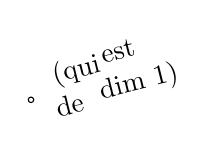
\begin{tikzpicture}[x=1cm,y=1cm]
  \draw (-0.18,-0.12) circle (0.035);
  \node[anchor=base west,rotate=14] at (0,0.06) {(qui};
  \node[anchor=base west,rotate=14] at (0.62,0.31) {est};
  \node[anchor=base west,rotate=14] at (0.05,-0.37) {de};
  \node[anchor=base west,rotate=14] at (0.60,-0.14) {dim $1$)};
\end{tikzpicture}}}}\normalmarginpar
% Left marginal insertion: est stands above/right of (qui; de stands lower/left of dim 1).
sont des éléments réguliers.
\margin{\handwritten{\figure{
\begin{tikzpicture}[x=1cm,y=1cm]\draw (-0.16,0.05)--(0,0)--(0,-2.05)--(-0.16,-2.08);\end{tikzpicture}}}}

\uline{Corollaire}\handwritten{1}: Soit $\handwritten{\mu}$ le sous-groupe de $W$ engendré par un élément de Coxeter $c$, donc $\handwritten{\mu\simeq}\underline{Z}\handwritten{/}h\underline{Z}$. Alors $\handwritten{\mu}$ est égal au centralisateur de $c$, donc de $\handwritten{\mu}$, et si $\handwritten{\nu}$ est le normalisateur de $\handwritten{\mu}$, l'homomorphisme
\reversemarginpar\margin{\handwritten{\figure{\begin{tikzpicture}[x=1cm,y=1cm]\draw (0,0)--(0,-2.4);\end{tikzpicture}}}}\normalmarginpar
\[
\handwritten{\unsure{\psi|\nu}/\mu\longrightarrow}\operatorname{Aut}(\handwritten{\mu})\handwritten{\simeq}(\underline{Z}/h\underline{Z})^{\handwritten{*}}
\]
\margin{\handwritten{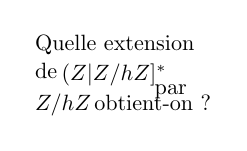
\begin{tikzpicture}[x=1cm,y=1cm,scale=0.80,transform shape]
  \node[anchor=base west] at (0,0.95) {Quelle extension};
  \node[anchor=base west] at (0,0.50) {de};
  \node[anchor=base west] at (0.42,0.48) {$(\unsure{Z|\mathbb{Z}}/hZ]^*$};
  \node[anchor=base west] at (1.90,0.25) {par};
  \node[anchor=base west] at (0,0) {$\mathbb{Z}/h\mathbb{Z}$};
  \node[anchor=base west] at (0.94,0) {obtient-on ?};
\end{tikzpicture}}}
est \unsure{un} isomorphisme; en d'autres termes, pour tout entier $n$ premier à $h$, il existe un $w\handwritten{\in}W$ tel que $wcw^{-1}=c^h$, et $w$ est déterminé mod $\handwritten{\mu}$.
\reversemarginpar\margin{\handwritten{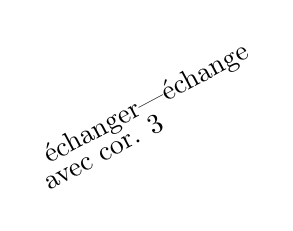
\begin{tikzpicture}[x=1cm,y=1cm]
  \node[anchor=base west,rotate=28] at (0,0.24) {\unsure{échanger|échange}};
  \node[anchor=base west,rotate=28] at (0,-0.10) {avec cor. $3$};
\end{tikzpicture}}}\normalmarginpar
% Slanted note in the left margin; no additional question mark follows the 3.

Soit \unsure{en} ef\deleted{\unsure{i}}\inserted{f}et $D$ \deleted{\unsure{une droite}}\inserted{le sous-espace} propre sous $c$ correspondant à une racine primitive $h$.ème de $1$. Alors $\dim D=1$ (prop.\handwritten{30}), et $\handwritten{\unsure{\mathfrak{z}|z}}=\operatorname{Centr}(\handwritten{\mu})$ normalise $D$, d'où un homomorphisme $\handwritten{\mathfrak{z}\to}\operatorname{Aut}(D)=\underline{C}^{\handwritten{*}}$, dont l'image est un sous-groupe fini de $\underline{C}^{\handwritten{*}}$, contenant l'image (isomorphe) de $\handwritten{\mu}$, donc cyclique d'ordre un multiple de $h$. Grâce à Kostant, son ordre est égal à $h$, et on a donc trouvé une rétraction $\handwritten{\mathfrak{z}\to\mu}$, il faut prouver que son noyau est réduit à $1$. Or si $w$ est dans ce noyau, il \deleted{induit} centralise $D$, et q\unsure{ô|ö}mme $D$ est régulière par Kostant,cela implique $w=1$. \unsure{Bn|On} a donc prouvé $\handwritten{\mathfrak{z}}=\handwritten{\mu}$. Reste à prouver que si $n$ est un entier premier à $h$, alors $c^n$ est conjugué de $c$, ce qui résulte également de Kostant.
% Each centralizer glyph combines a typed z-shaped upper part with a handwritten lower loop.

\uline{Corollaire}. Soit $c$ un élément de Coxeter, et $\handwritten{\lambda}$ une valeur propre de $c$, correspondant à un vecteur propre $x$. Pour que $x$ soit régulier, il faut et il suffit que $\handwritten{\lambda}$ soit une racine primitive $h$.ème de $1$.
\reversemarginpar\margin{\handwritten{\figure{
\begin{tikzpicture}[x=1cm,y=1cm]\draw (0.05,0)--(0,-0.15)--(0,-1.05);\end{tikzpicture}}}}\normalmarginpar

La suffisance a déjà été énoncée avec le th. de Kostant. Pour la nécessité, soit $h'\handwritten{\leq}h$ l'ordre de la valeur propre, alors $\unsure{\mathbin{.}|}c^{h'}$ centralise $x$, donc, $x$ étant régulier, on a $c^{h'}=1$, donc $h'=h$, cqfd.

\uline{Corollaire}. 
\begin{tikzpicture}[baseline=(live.base),x=1cm,y=1cm]
  \node[anchor=base west,inner sep=0pt] at (0.15,0.39) {\deleted{\unsure{Considérons}}};
  \node[anchor=base west,inner sep=0pt] (live) at (0,0.14) {\inserted{Soit $D$ une}};
  \node[anchor=base west,inner sep=0pt] at (0,-0.12) {\deleted{Soit $D$ une}};
\end{tikzpicture} droite régulières dans $V\mathbin{\text{\textcircled{x}}}\underline{C}$ telle qu'il existe un élé%
% archive sheet number: 1
